\subsection{Was ist die Flexcloud?} \setauthor{Pouget Marcel}





Die Flexcloud, auch FlexcommunicationCloud genannt, ist eine Erfindung der Firma FlexSolution. Die Anwendung findet im Firmeneigenen Netzwerk statt, und ermöglicht es, viele kleine Microservices miteinander kommunizieren zu lassen. Die Hauptkomponente, der sogenannte FlexCore, wurde von den Mitarbeitern in der Sprache Java entwickelt. Mit der sogenannten Flexlib lassen sich die Anwendungen mit vielen weiteren kleinen Dependencies erweitern. Das wird vor allem dann benötigt, wenn z.B. eine Datenbankanbindung notwendig ist. Die Flexcloud besteht also aus lauter sogenannten Flextasks, welche verschiedene Aufgaben ausführen. Siehe \ref{fig:impl:FlexcloudAnsicht}. Es zum Beispiel einen Task, der für die Ansteuerung der Lampen und Rollos zuständig ist.

\begin{figure}[h t]
    \centering
    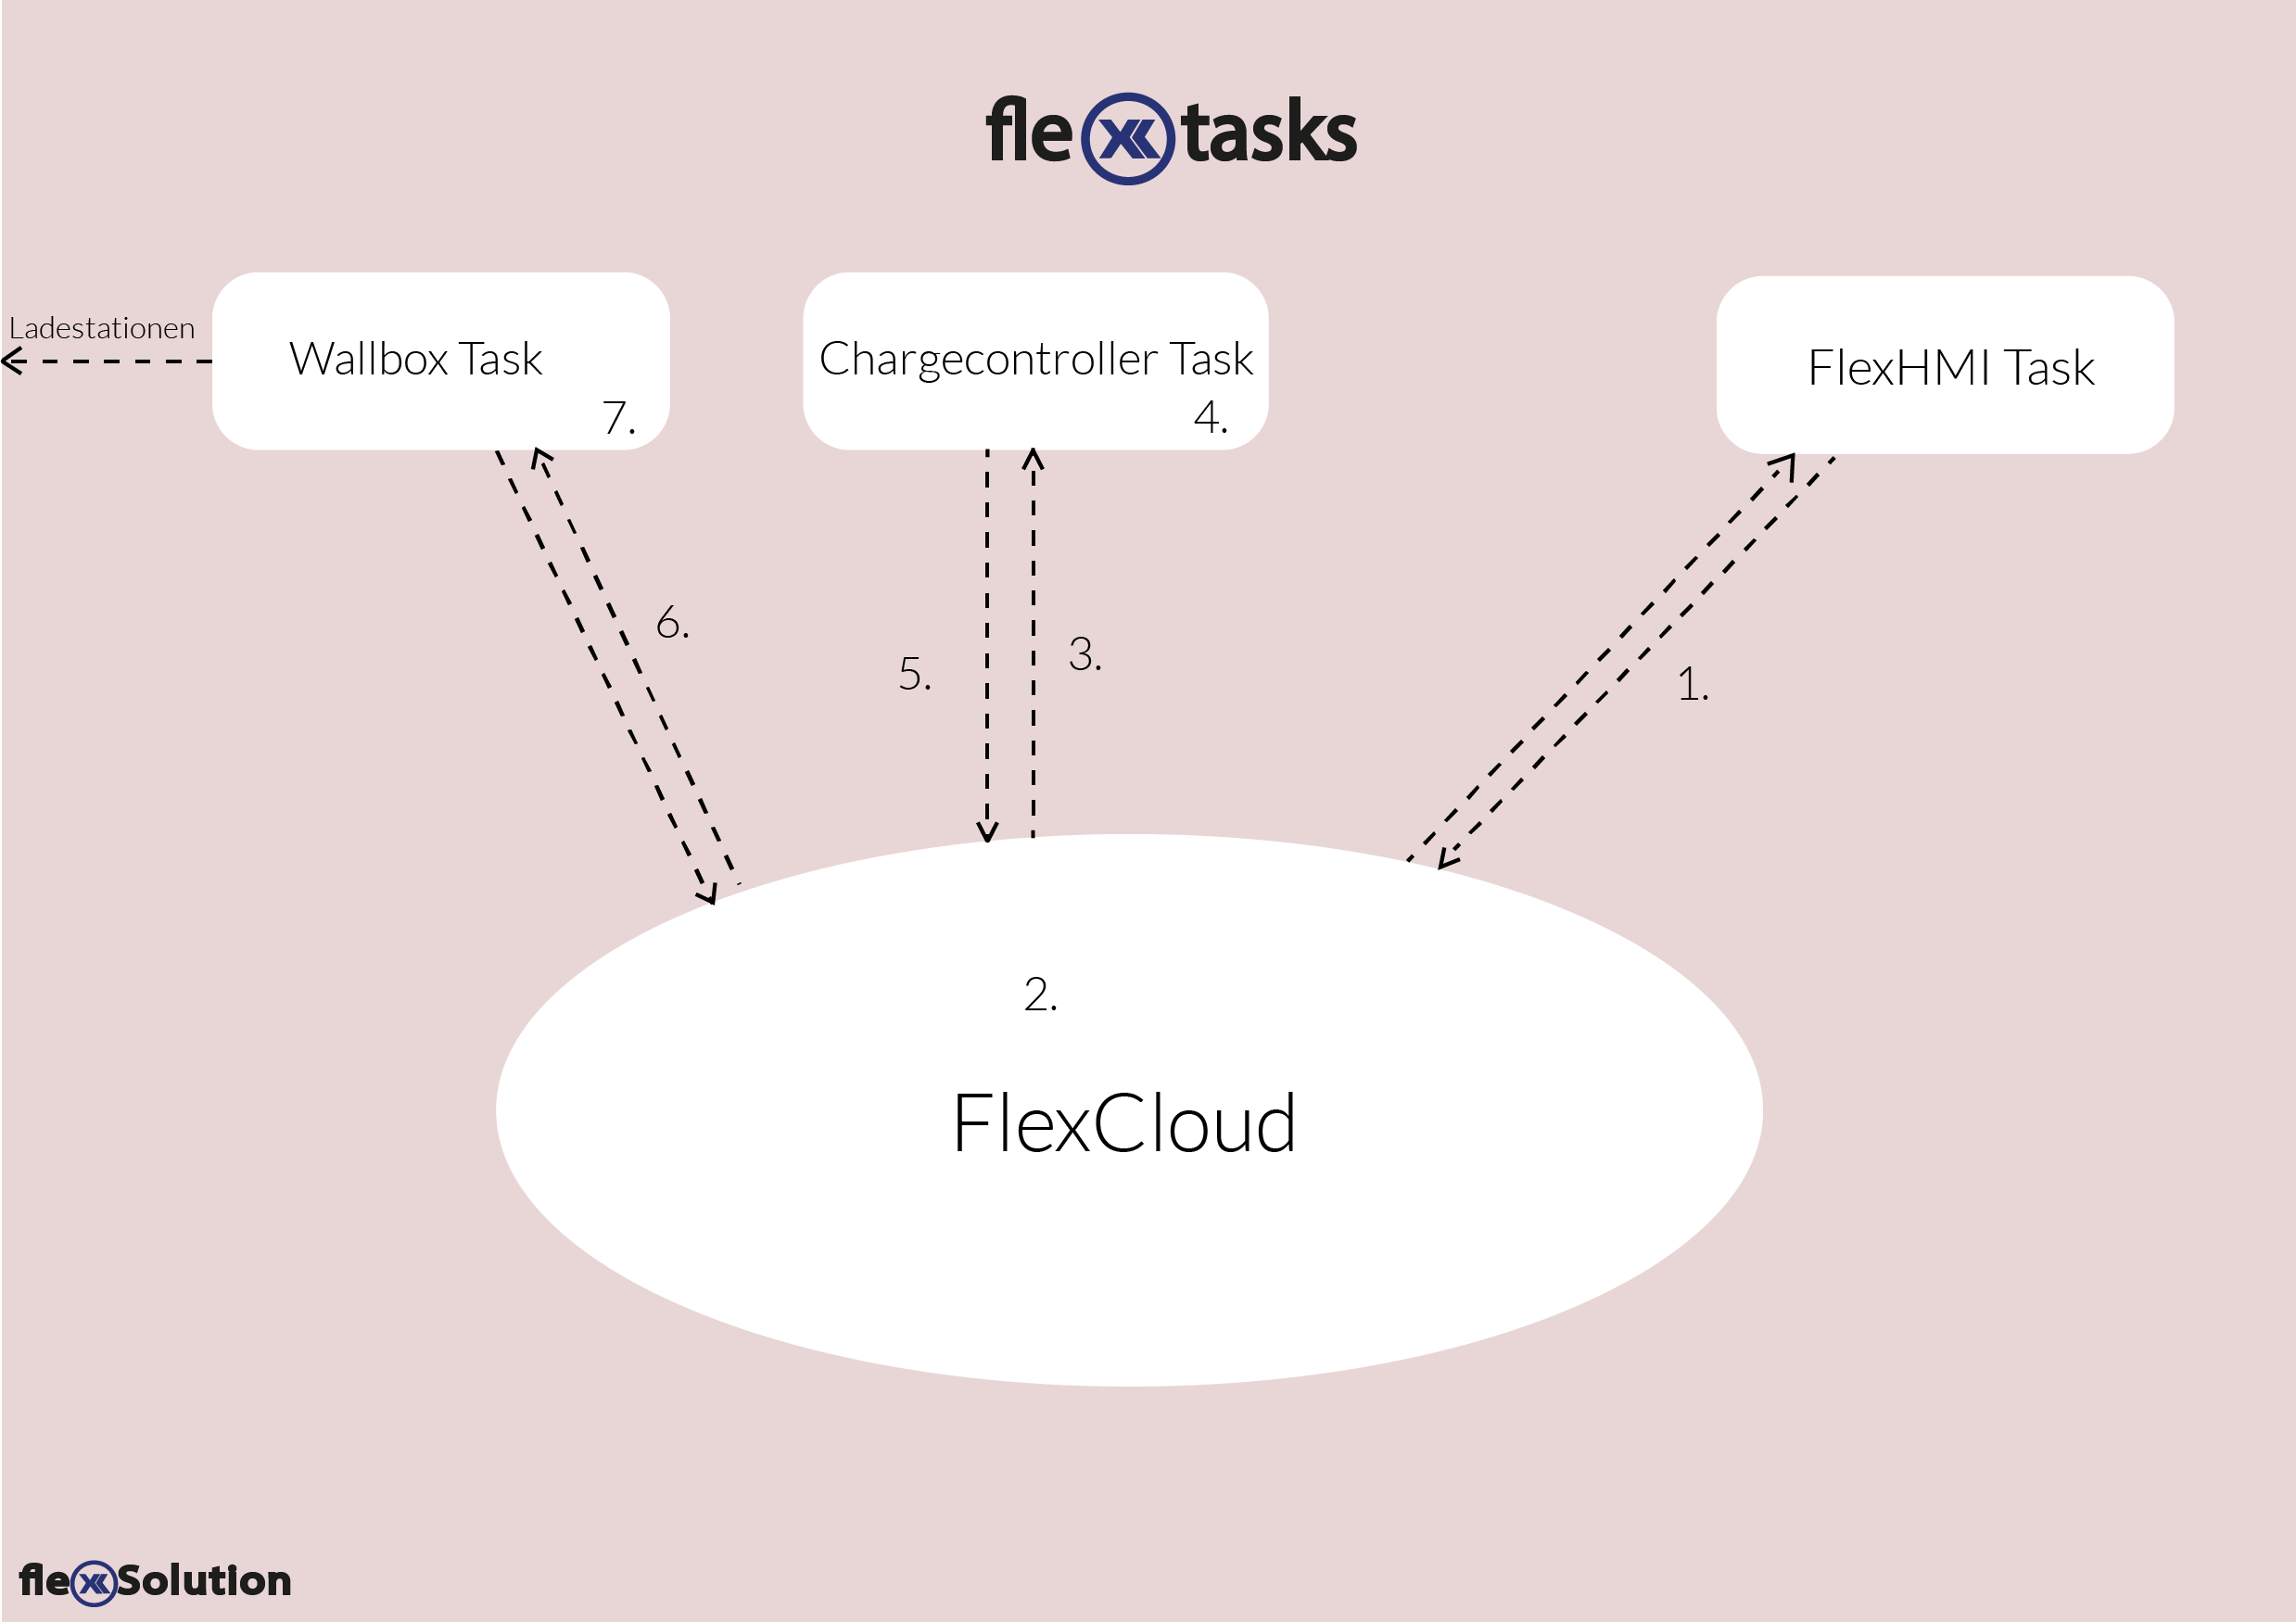
\includegraphics[scale=0.7]{pics/flexTasks2.png}
    \caption{Darstellung des Aufbaues}
    \label{fig:impl:FlexcloudAnsicht}
\end{figure}




Ein weiterer Task, der für die HMI zuständig ist, verbindet die Flexcloud mit dem Browser. Die FlexcommunicationCloud ist auch für viele kleinere Anwendungen nützlich, da sich solche Microservices sehr schnell aufsetzen lassen. Man kann einzelne Tasks aufsetzen oder mehrere miteinander verbinden und kommunizieren lassen. Das hat den Vorteil, dass man wiederverwendbare Anwendungen entwickeln kann, welche nur grundlegende Funktionen erfüllen, aber von vielen Tasks gebraucht werden. So ist es z.B. in Planung, einen eigenen Modbus-Task zu implementieren, welcher nur dafür da ist, Befehle von anderen Tasks zu übernehmen und an eine USB-Schnittstelle weiterzuleiten.
Damit die Tasks untereinander kommunizieren können, hat die Firma die sogenannten Datenpunkte (Datapoints) entwickelt. Sie dienen dazu, um zwischen einem oder mehreren Tasks Informationen oder Werte auszutauschen. Auch Funktionen-Aufrufe können durch solche Datapoints ermöglicht werden. Um durch Datenpunkte miteinander zu kommunizieren, müssen besagte FlexTasks mit den Project\_ID's verbunden werden.
Wie man die Datenpunkte anlegen kann, was dabei wichtig ist und wie die Daten gemapped werden, wird im Kapitel \ref{Datenpunkte} beschrieben.
\subsection{Grundaufbau der Tasks}

\begin{compactenum}

    \item Pom.xml des Tasks editieren: Als erstes sollte die MainClass gesetzt werden. Dies folgt immer einem gewissen Schema. Die Klasse sollte im Package 'eu.flexsolution.task.' zu finden sein. Die GroupID ist dieselbe wie das Package der MainClass. In dem Fall ist es wieder 'eu.flexsolution.task'.  In der 'artifactId' steht der Name des Tasks. Bei den Dependencies wird der 'Flexsolution core', 'log4j', 'org.json'. Eine weiter wichtige Sache ist das Einbinden des 'Internal Snapshot Repository'. Das ist der Ort, an dem der Flexsolution core und die Flexlib gepublished werden. Maven lädt dann beim Starten der Applikation die Dependencies von dem von der Firma bereitgestellten Server herunter, und fügt sie zur Applikation hinzu.
    \item Das Anlegen der Main Klasse. Der erste Schritt ist, die Klasse 'FlexTask' zu erweitern.
    \begin{lstlisting}[language=java,caption=Erweiterung einer Java-Klasse mit einem 'Flextask',label=lst:impl:foo]
        public class FlexTaskModbuswallbox extends FlexTask 
    \end{lstlisting}
    Dadurch werden einige Funktionen überschrieben, bei denen die meisten jedoch nicht verwendet werden. In der 'public static void main' wird ein neues Objekt der Main Klasse erstellt.
    \begin{lstlisting}[language=java,caption=Aufruf eines neuen Objektes der Klasse FlexTaskModbusWallbox,label=lst:impl:foo]
        new FlexTaskModbuswallbox();  
    \end{lstlisting}
    In der 'initTask(){}' Methode kann dann die Hauptfunktion des Tasks implementiert werden. In den meisten Fällen werden hierfür Datenpunkte und andere Kommunikations-Methoden eingebunden. Mit Fertigstellung der App muss der Code mithilfe von Maven zu einem JAR-File kompiliert werden.

    \item Linux-Maschine vorbereiten: Als erster Schritt ist es wichtig, ein Verzeichnis für den Task zu erstellen. In diese wird dann das .jar File kopiert. Da in der Firma mit 'log4j' gearbeitet wird, muss hierfür noch ein Konfigurations-File angelegt werden. (siehe log4j File)
    Da jeder Flextask eine Datenbank mit den für ihn zugehörigen Datenpunkten besitzt, muss dieses File auch erst angelegt und konfiguriert werden: im Verzeichnis ‘/var/flex/tasks/’ wird ein neuer Ordner mit dem Namen des Tasks angelegt. In diesem wird die Datei conf.db erstellt und folgende Tabellen hinzugefügt:
    \begin{lstlisting}[language=java,caption=Log4J File,label=lst:impl:foo]
        [Service]
        Type=simple
        ExecStart=/usr/bin/java -Xmx32m -Dlog4j.configurationFile=./log4j2.xml -jar /srv/tasks/CURRENT/modbuswallbox/modbuswallbox.jar
        Environment="TASKNAME=modbuswallbox"
        WorkingDirectory=/srv/tasks/CURRENT/modbuswallbox
        TimeoutStopSec=3
        Restart=always
        RestartSec=10
        Slice=flexTasks.slice
        [Install]
        WantedBy=default.target
    \end{lstlisting}
    \item Da jeder Flextask eine Datenbank mit den für ihn zugehörigen Datenpunkten besitzt, muss dieses File auch erst angelegt und konfiguriert werden: im Verzeichnis ‘/var/flex/tasks/’ wird ein neuer Ordner mit dem Namen des Tasks angelegt. In diesem wird die Datei conf.db erstellt und folgende Tabellen hinzugefügt:
    \begin{compactenum}
        \item Device: besteht aus einer 'ID' und einem Label. Im Falle des Gateways sind es 5 Geräte, für jede Wallbox eines. Das ist dafür gut, um Datenpunkte mit denselben Namen nutzen zu können, da man sie mithilfe der Deviceid unterschieden kann
        \item DeviceParameter: Hier können wichtige Parameter gesetzt werden, die dann beim Starten eines Tasks mit der Methode 'getNeededDeviceParameters(Map<String, ValueCheck> map)'ausgelesen werden können. Die Tabelle besteht aus einer ID, einer DeviceID, einem Wert und einem Label.
        \item taskParameter: hier können wichtige Parameter für das System gesetzt werden. Meistens wird hier nur der Standard-Port 8150 gesetzt. Die Tabelle besteht aus einer Spalte für die ID, für Values und einer für Labels. Auch hier können beim Starten eines Tasks die Werte der DB ausgelesen werden. Hierfür verwendet man die Funktion 'getNeededTaskParameters(Map<String, ValueCheck> map)'.
        \item datapoint\_valueMapping: Besteht aus einer Datapoint1\_id und Datapoint2\_id, einem Wert und einer Spalte für neue Werte (new\_Value). Dies ist dafür da, um zwischen zwei Datenpunkten die Werte zu synchronisieren oder gegebenenfalls mit new\_Value zu überschreiben
        \item Datapoint: Herzstück der Datenbank. Hier werden die Datenpunkte angelegt \ref{Datenpunkte}. Die Tabelle besteht aus einer ID, einer device\_id, einem Label, einer 'specificAddress', einem 'specificDatatype', einem 'specificStruct', einem Datentyp (datatype), Flags, einem Intervall, einem Threshold und einer Value. Für das Starten des Tasks ist diese Tabelle zu befüllen, jedoch ist sie unumgänglich, wenn man die Hauptfunktionen der Flexlib verwenden möchte
        \item datapoint\_map: Diese Tabelle besteht aus einer datapoint1\_id, einer datapoint2\_id und einer Funktion. Diese Tabelle wird dazu verwendet, um Zwei Datenpunkte zu mappen (verknüpfen).
        \item SystemParameter: Hier werden die wichtigsten Einstellungen für den Task selbst getroffen. Es gibt Einstellungen für den Namen des Tasks, den Port und man kann das keep\_Alive Signal einstellen. Außerdem gibt es die PROJECT\_ID, welche für das Verbinden mehrerer Tasks notwendig ist. Denn es können sich nur FlexTasks finden, welche dieselbe Project\_ID besitzen. Im Falle des Gateways werden die Tasks mit der ID 'AUT, HMI, chargecontroller' verbunden. Das ist wichtig, um den einzelnen Tasks die benötigten Parameter zu übergeben. AUT ist in dem Fall die Haussteuerung, HMI ist der oben kurz beschriebene Flextask zur Veranschaulichung der Elemente und chargecontroller ist der auch schon beschriebene Controller für dieses Projekt.
    \end{compactenum}
    \item Wenn alle Pfade richtig benannt wurden, kann man im Verzeichnis einen symbolischen Link zu dem .jar-File machen. Das hilft bei der Entwicklung, da man bei einer Namensänderung nur den Link anpassen muss und nicht die angegebenen Pfade in den Konfigurations-Dateien.
    \item Starten, stoppen bzw. überwachen kann man den Task mit 'systemctl --user start / stop / restart / status FlextasName.service
    \item Mit dem Command 'tail -f /tmp/log/ FlextaskName.log' kann man in Echtzeit mitansehen, was Log4j in das File schreibt. Die Files werden alle in dem Verzeichnis '/tmp/log/' gespeichert, wenn sie nach einiger Zeit nicht mehr benötigt werden, werden sie komprimiert und in ein anderes Verzeichnis verschoben, um Platz zu sparen.
\end{compactenum}
